
\medskip

%On a construit un bac à sable pour enfants.
%\begin{center}
%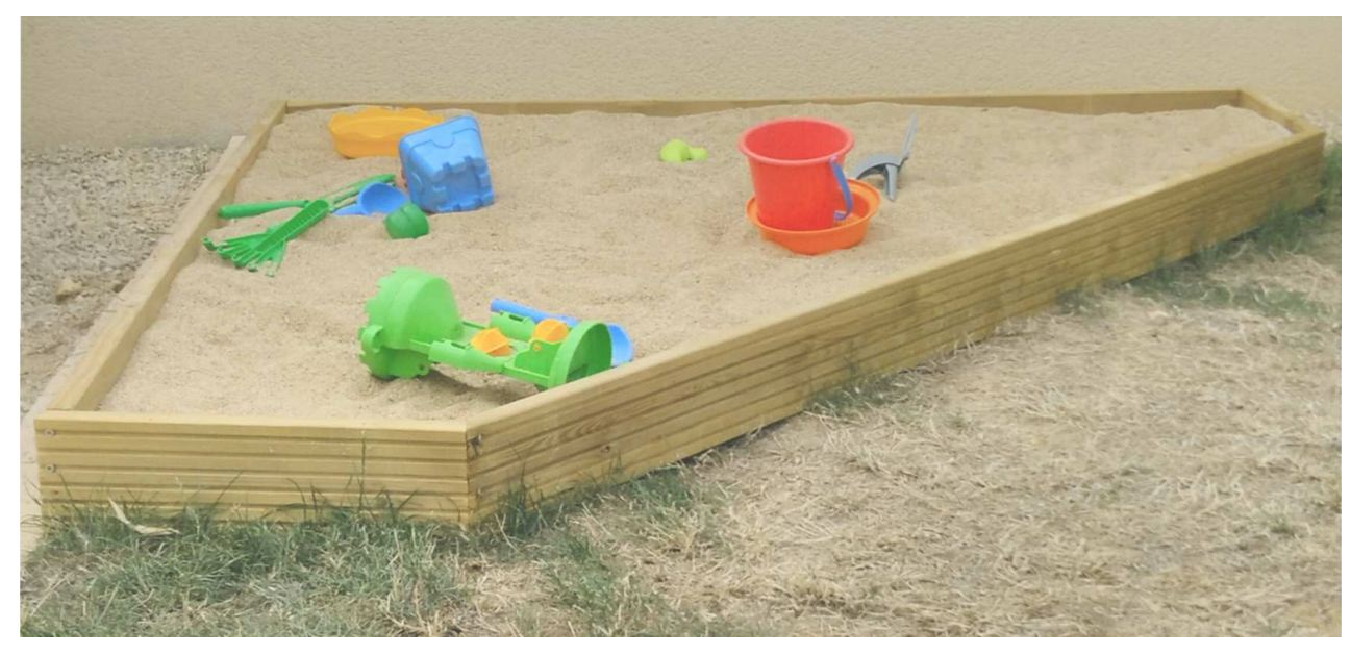
\includegraphics[width=10cm]{bac_a_sable}
%\end{center}
%
%Ce bac a la forme d'un prisme droit de hauteur $15$ cm. La base de ce prisme droit est représentée
%par le polygone ABCDE ci-dessous:
%
%\smallskip
%
%\emph{Attention la figure n'est pas construite à la taille réelle}.
%
%\smallskip
%
%\begin{minipage}{0.48\linewidth}
%On donne :
%\begin{itemize}
%\item PC = PD = 1,30 m
%\item ED = BC = 40 cm
%\item E, D, P sont alignés
%\item B, C, P sont alignés
%\end{itemize}
%\end{minipage}
%\hfill \begin{minipage}{0.48\linewidth}
%\begin{pspicture}(5.5,5.5)
%\pspolygon(2.5,0.5)(0.5,0.5)(0.5,5)(5,5)(5,3)%DEABCD
%\psline[linestyle=dashed](5,3)(5,0.5)(2.5,0.5)
%\psframe(0.5,0.5)(0.7,0.7)\psframe(0.5,5)(0.7,4.8)
%\psframe(5,5)(4.8,4.8)\psframe(5,0.5)(4.8,0.7)
%\uput[ul](0.5,5){A} \uput[ul](0.5,0.5){E} \uput[ur](5,5){B} 
%\uput[r](5,3){C} \uput[d](2.5,0.5){D} \uput[dr](5,0.5){P}
%\psline(1.5,0.4)(1.5,0.6) \psline(4.9,4)(5.1,4)
%\psline(3.73,0.4)(3.73,0.6)\psline(3.77,0.4)(3.77,0.6)
%\psline(4.9,1.73)(5.1,1.73)\psline(4.9,1.77)(5.1,1.77)
%\end{pspicture}
%\end{minipage}
%
%\smallskip

\begin{enumerate}
\item %Calculer CD. Arrondir au centimètre près.
Dans le triangle PCD, rectangle isocèle en P le théorème de Pythagore s'écrit :

CD$^2 = \text{PC}^2 + \text{PD}^2 = 1,3^2 + 1,3^2 = 3,38$, d'où CD $= \sqrt{3,38} \approx 1,838$, soit 1,84~(m) au centimètre près.
\item %Justifier que le quadrilatère ABPE est un carré.
ABPE a quatre angles droits : c'est donc un rectangle.

PE $ = \text{PD} + \text{DE} = 1,30 + 0,40 = 1,7$~(m) ;


PB $ = \text{PC} + \text{CB} = 1,30 + 0,40 = 1,7$~(m).

Le quadrilatère est un rectangle qui a deux côtés consécutifs de même longueur, c'est donc un losange et un carré. 
\item %En déduire le périmètre du polygone ABCDE. Arrondir au centimètre près.
Le périmètre du bac est donc égal approximativement à :

$\text{AB} + \text{BC} + \text{CD} + \text{DE} + \text{EA} = 1,7 + 0,4 + 1,84 + 0,4 + 1,7$ soit 6,04~(m).
\item %On a construit le tour du bac à sable avec des planches en bois de longueur $2,40$~m et
%de hauteur $15$~cm chacune. De combien de planches a-t-on eu besoin?
La hauteur est suffisante. En longueur deux planches ne suffisent pas  ; trois suffisent 

($3 \times 2,40 = 7,20 > 6,04$).
\item %Calculer, en m$^2$, l'aire du polygone ABCDE.
$\mathcal{A}(\text{ABCDE}) = \mathcal{A}(\text{ABPE}) - \mathcal{A}(\text{CPD}) = 1,7^2 - \dfrac{1,3 \times 1,3}{2} = 2,89 - 0,845 = 2,045$~$\left(\text{m}^2\right)$.
\item %A-t-on eu besoin de plus de $300$~L de sable pour remplir complètement le bac ?
Le volume du bac est égal environ à :

$2,045 \times 0,15 = \np{0,30675}~\left(\text{m}^3\right)$.

or 1~m$^3 = \np{1000}$~dm$^3 = \np{1000}$~(L).

Donc le volume du bac en litres est égal environ à :

$\np{0,30675} \times \np{1000} = 306,75$~(L), soit plus de 300~(L) de sable.
\end{enumerate}
%\begin{center}
%\emph{Rappel : Volume d'un prisme droit $=$ aire de la base $\times$ hauteur}
%\end{center}


